%%%%%%%%%%%%%%%%%%%%%%%%%%%%%%%%%%%%%%%%%%%%%
%%%%%%%%%%%%%%%%%%%%%%%%%%%%%%%%%%%%%%%%%%%%%
% delete the stuff here when we compile the whole book
\documentclass{book}

\usepackage{fancyhdr}
\pagestyle{fancy}

\renewcommand{\chaptername}{Laboratory}
\usepackage{amsfonts}
\usepackage{times}
\usepackage[pdftex]{graphicx}
%\DeclareGraphicsExtensions{.jpg}
%\usepackage[dvips]{graphicx}
%\DeclareGraphicsExtensions{.eps}
\usepackage{latexsym}
\usepackage{amssymb}
\usepackage{amsmath}
\usepackage{mathabx}
\usepackage{cite}
\usepackage{verbatim}
\usepackage[outdir=./]{epstopdf}
\usepackage{bm}
\usepackage{cancel}
\usepackage{color}
\usepackage{wrapfig}
\usepackage{listings} % alternative to verbatim package
\lstset{
basicstyle=\small\ttfamily,
columns=flexible,
breaklines=true
}
\usepackage[pdftex]{hyperref} % added to make clickable URLS


\newtheorem{theorem}{Theorem}

\newtheorem{acknowledgement}[theorem]{Acknowledgement}
\newtheorem{algorithm}[theorem]{Algorithm}
\newtheorem{assumption}[theorem]{Assumption}
\newtheorem{axiom}[theorem]{Axiom}
\newtheorem{case}[theorem]{Case}
\newtheorem{claim}[theorem]{Claim}
\newtheorem{conclusion}[theorem]{Conclusion}
\newtheorem{condition}[theorem]{Condition}
\newtheorem{conjecture}[theorem]{Conjecture}
\newtheorem{corollary}[theorem]{Corollary}
\newtheorem{criterion}[theorem]{Criterion}
\newtheorem{definition}[theorem]{Definition}
\newtheorem{example}[theorem]{Example}
\newtheorem{exercise}[theorem]{Exercise}
\newtheorem{fact}[theorem]{Fact}
\newtheorem{lemma}[theorem]{Lemma}
\newtheorem{notation}[theorem]{Notation}
\newtheorem{problem}[theorem]{Problem}
\newtheorem{proposition}[theorem]{Proposition}
\newtheorem{solution}[theorem]{Solution}
\newtheorem{summary}[theorem]{Summary}
\newtheorem{remark}[theorem]{Remark}
\newenvironment{proof}{ \textbf{Proof:} }{ \hfill $\Box$}
  
\newcommand{\figref}[1]{{Fig.}~\ref{#1}}
\newcommand{\secref}[1]{{Section}~\ref{#1}}
\newcommand{\exref}[1]{{Example}~\ref{#1}}
\newcommand{\tabref}[1]{{Table}~\ref{#1}}
\newcommand{\eref}[1]{(\ref{#1})}
\newcommand{\bookemph}[1]{ {\em #1}}
\newcommand{\Ns}{N_{\mathrm{s}}}
\newcommand{\Ut}{U_\mathrm{t}}
\newcommand{\fig}[1]{Fig.\ \ref{#1}}
\def\onehalf{\frac{1}{2}}
\def\etal{et.\/ al.\/}
\newcommand{\bydef}{\triangleq}

% Specific additions for the wireless lab
\newcommand{\turnin}[1]{\noindent \fbox{\parbox{\linewidth}{\textbf{Turn in:} #1}}}
\newcommand{\showta}[1]{\noindent \fbox{\parbox{\linewidth}{\textbf{Show the TA:} #1}}}

\def\Trans {{\rm T}}
\def\Conj {{\rm c}}
\def\tr {{\rm tr}}
\def\E{{\mathbb E}}
\def\P{{\mathbb P}}
\def\phase{\mathrm{phase}}
\def\Mt{{M_\mathrm{t}}}
\def\Mr{{M_\mathrm{r}}}
\def\Ns{{N_\mathrm{s}}}
\def\Nt{{N_\mathrm{t}}}
\def\Ntot{{N_\mathrm{tot}}}
\def\Nbuf{{N_\mathrm{buf}}}
\def\Ntr{{N_\mathrm{tr}}}
\def\Nr{{N_\mathrm{r}}}
\def\Ne{{N_\mathrm{e}}}
\def\Ns{{N_\mathrm{s}}}
\def\Np{{N_\mathrm{p}}}
\def\Nc{{N_\mathrm{c}}}
\def\Ng{{N_\mathrm{g}}}
\def\Es{{E_\mathrm{s}}}
\def\Ex{{E_\mathrm{x}}}
\def\No{{N_\mathrm{o}}}
\def\Lc{{L_\mathrm{c}}}
\def\Lt{{L_\mathrm{t}}}
\def\Lp{{L_\mathrm{p}}}
\def\Lf{{L_\mathrm{f}}}
\def\nd{{n_\mathrm{d}}}
\def\sinc{\mathrm{sinc}}
\def\dmin{d_{\mathrm{min}}}
%\def\dmin2{d^2_{\mathrm{min}}}
\def\vecc{\mathrm{vec}} % changed it to vec to not overwrite \vec from amsmath
\def\kron{\otimes}
\def\onehalf{\frac{1}{2}}
\def\Rdelay{R_{\mathrm{delay}}}
\def\Rdoppler{R_{\mathrm{Doppler}}}
\def\Bc{B_{\mathrm{coh}}}
\def\Tc{T_{\mathrm{coh}}}
\def\Sdelay{\sfS_{\mathrm{delay}}}
\def\Sdoppler{\sfS_{\mathrm{Doppler}}}
\def\gtx{g_{\mathrm{tx}}}
\def\Gtx{G_{\mathrm{tx}}}
\def\grx{g_{\mathrm{rx}}}
\def\sigmaRMSdelay{\sigma_{\mathrm{RMS,delay}}}
\def\sigmaRMSdoppler{\sigma_{\mathrm{RMS,doppler}}}
\def\Grx{G_{\mathrm{rx}}}
\def\SNR{\mathrm{SNR}} % note that I changed this
\def\SINR{\mathrm{SINR}} % note that I changed this
\def\ExNo{\frac{E_{\mathrm{x}}}{N_{\mathrm{o}}}}
\def\bargtx{\bar{g}_{\textrm{tx}}}
\DeclareMathOperator*{\argmin}{arg\,min}
\DeclareMathOperator*{\argmax}{arg\,max}
\def\Gauss{{\mathcal{N}}}
\def\GaussComp{{\mathcal{N}_\mathbb{C}}}
\def\Pe{P_{\mathrm{e}}}
\def\dB{\mathrm{dB}}
\def\dBm{\mathrm{dBm}}
\def\Watt{\mathrm{W}}
\def\mWatt{\mathrm{mW}}
\def\DeltaTime{\Delta_{\mathrm{time}}}
\def\DeltaFreq{\Delta_{\mathrm{freq}}}
\def\DeltaLag{\Delta_{\mathrm{lag}}}
\def\Rtime{R_{\mathrm{time}}}
\def\Rlag{R_{\mathrm{lag}}}
\def\wtrain{w_{\text{train}}}
\def\DFT{\text{DFT}}
\def\IDFT{\text{IDFT}}



% blackboard lowercase
\def\bydef{:=}
\def\bba{{\mathbb{a}}}
\def\bbb{{\mathbb{b}}}
\def\bbc{{\mathbb{c}}}
\def\bbd{{\mathbb{d}}}
\def\bbee{{\mathbb{e}}}
\def\bbff{{\mathbb{f}}}
\def\bbg{{\mathbb{g}}}
\def\bbh{{\mathbb{h}}}
\def\bbi{{\mathbb{i}}}
\def\bbj{{\mathbb{j}}}
\def\bbk{{\mathbb{k}}}
\def\bbl{{\mathbb{l}}}
\def\bbm{{\mathbb{m}}}
\def\bbn{{\mathbb{n}}}
\def\bbo{{\mathbb{o}}}
\def\bbp{{\mathbb{p}}}
\def\bbq{{\mathbb{q}}}
\def\bbr{{\mathbb{r}}}
\def\bbs{{\mathbb{s}}}
\def\bbt{{\mathbb{t}}}
\def\bbu{{\mathbb{u}}}
\def\bbv{{\mathbb{v}}}
\def\bbw{{\mathbb{w}}}
\def\bbx{{\mathbb{x}}}
\def\bby{{\mathbb{y}}}
\def\bbz{{\mathbb{z}}}
\def\bbone{{\mathrm{I}}}

% Bold lowercase
\def\bydef{:=}
\def\ba{{\mathbf{a}}}
\def\bb{{\mathbf{b}}}
\def\bc{{\mathbf{c}}}
\def\bd{{\mathbf{d}}}
\def\bee{{\mathbf{e}}}
\def\bff{{\mathbf{f}}}
\def\bg{{\mathbf{g}}}
\def\bh{{\mathbf{h}}}
\def\bi{{\mathbf{i}}}
\def\bj{{\mathbf{j}}}
\def\bk{{\mathbf{k}}}
\def\bl{{\mathbf{l}}}
\def\bmm{{\mathbf{m}}} % changed to avoid conflict with bold
\def\bn{{\mathbf{n}}}
\def\bo{{\mathbf{o}}}
\def\bp{{\mathbf{p}}}
\def\bq{{\mathbf{q}}}
\def\br{{\mathbf{r}}}
\def\bs{{\mathbf{s}}}
\def\bt{{\mathbf{t}}}
\def\bu{{\mathbf{u}}}
\def\bv{{\mathbf{v}}}
\def\bw{{\mathbf{w}}}
\def\bx{{\mathbf{x}}}
\def\by{{\mathbf{y}}}
\def\bz{{\mathbf{z}}}
%\def\b0{{\mathbf{0}}}
%\def\b1{{\mathbf{1}}}
\def\bzero{{\mathbf{0}}}
\def\bone{{\mathbf{1}}}
\def\NLF{N_{\mathrm{LF}}}
% Bold capital letters
\def\bA{{\mathbf{A}}}
\def\bB{{\mathbf{B}}}
\def\bC{{\mathbf{C}}}
\def\bD{{\mathbf{D}}}
\def\bE{{\mathbf{E}}}
\def\bF{{\mathbf{F}}}
\def\bG{{\mathbf{G}}}
\def\bH{{\mathbf{H}}}
\def\bI{{\mathbf{I}}}
\def\bJ{{\mathbf{J}}}
\def\bK{{\mathbf{K}}}
\def\bL{{\mathbf{L}}}
\def\bM{{\mathbf{M}}}
\def\bN{{\mathbf{N}}}
\def\bO{{\mathbf{O}}}
\def\bP{{\mathbf{P}}}
\def\bQ{{\mathbf{Q}}}
\def\bR{{\mathbf{R}}}
\def\bS{{\mathbf{S}}}
\def\bT{{\mathbf{T}}}
\def\bU{{\mathbf{U}}}
\def\bV{{\mathbf{V}}}
\def\bW{{\mathbf{W}}}
\def\bX{{\mathbf{X}}}
\def\bY{{\mathbf{Y}}}
\def\bZ{{\mathbf{Z}}}

% Blackboard capital letters
\def\bbA{{\mathbb{A}}}
\def\bbB{{\mathbb{B}}}
\def\bbC{{\mathbb{C}}}
\def\bbD{{\mathbb{D}}}
\def\bbE{{\mathbb{E}}}
\def\bbF{{\mathbb{F}}}
\def\bbG{{\mathbb{G}}}
\def\bbH{{\mathbb{H}}}
\def\bbI{{\mathbb{I}}}
\def\bbJ{{\mathbb{J}}}
\def\bbK{{\mathbb{K}}}
\def\bbL{{\mathbb{L}}}
\def\bbM{{\mathbb{M}}}
\def\bbN{{\mathbb{N}}}
\def\bbO{{\mathbb{O}}}
\def\bbP{{\mathbb{P}}}
\def\bbQ{{\mathbb{Q}}}
\def\bbR{{\mathbb{R}}}
\def\bbS{{\mathbb{S}}}
\def\bbT{{\mathbb{T}}}
\def\bbU{{\mathbb{U}}}
\def\bbV{{\mathbb{V}}}
\def\bbW{{\mathbb{W}}}
\def\bbX{{\mathbb{X}}}
\def\bbY{{\mathbb{Y}}}
\def\bbZ{{\mathbb{Z}}}

% Caligraphic capital letters
\def\cA{\mathcal{A}}
\def\cB{\mathcal{B}}
\def\cC{\mathcal{C}}
\def\cD{\mathcal{D}}
\def\cE{\mathcal{E}}
\def\cF{\mathcal{F}}
\def\cG{\mathcal{G}}
\def\cH{\mathcal{H}}
\def\cI{\mathcal{I}}
\def\cJ{\mathcal{J}}
\def\cK{\mathcal{K}}
\def\cL{\mathcal{L}}
\def\cM{\mathcal{M}}
\def\cN{\mathcal{N}}
\def\cO{\mathcal{O}}
\def\cP{\mathcal{P}}
\def\cQ{\mathcal{Q}}
\def\cR{\mathcal{R}}
\def\cS{\mathcal{S}}
\def\cT{\mathcal{T}}
\def\cU{\mathcal{U}}
\def\cV{\mathcal{V}}
\def\cW{\mathcal{W}}
\def\cX{\mathcal{X}}
\def\cY{\mathcal{Y}}
\def\cZ{\mathcal{Z}}

% Sans serif capital letters
\def\sfA{\mathsf{A}}
\def\sfB{\mathsf{B}}
\def\sfC{\mathsf{C}}
\def\sfD{\mathsf{D}}
\def\sfE{\mathsf{E}}
\def\sfF{\mathsf{F}}
\def\sfG{\mathsf{G}}
\def\sfH{\mathsf{H}}
\def\sfI{\mathsf{I}}
\def\sfJ{\mathsf{J}}
\def\sfK{\mathsf{K}}
\def\sfL{\mathsf{L}}
\def\sfM{\mathsf{M}}
\def\sfN{\mathsf{N}}
\def\sfO{\mathsf{O}}
\def\sfP{\mathsf{P}}
\def\sfQ{\mathsf{Q}}
\def\sfR{\mathsf{R}}
\def\sfS{\mathsf{S}}
\def\sfT{\mathsf{T}}
\def\sfU{\mathsf{U}}
\def\sfV{\mathsf{V}}
\def\sfW{\mathsf{W}}
\def\sfX{\mathsf{X}}
\def\sfY{\mathsf{Y}}
\def\sfZ{\mathsf{Z}}


% Bold sans serif capital letters
\def\bsfA{\bm{\mathsf{A}}}
\def\bsfB{\bm{\mathsf{B}}}
\def\bsfC{\bm{\mathsf{C}}}
\def\bsfD{\bm{\mathsf{D}}}
\def\bsfE{\bm{\mathsf{E}}}
\def\bsfF{\bm{\mathsf{F}}}
\def\bsfG{\bm{\mathsf{G}}}
\def\bsfH{\bm{\mathsf{H}}}
\def\bsfI{\bm{\mathsf{I}}}
\def\bsfJ{\bm{\mathsf{J}}}
\def\bsfK{\bm{\mathsf{K}}}
\def\bsfL{\bm{\mathsf{L}}}
\def\bsfM{\bm{\mathsf{M}}}
\def\bsfN{\bm{\mathsf{N}}}
\def\bsfO{\bm{\mathsf{O}}}
\def\bsfP{\bm{\mathsf{P}}}
\def\bsfQ{\bm{\mathsf{Q}}}
\def\bsfR{\bm{\mathsf{R}}}
\def\bsfS{\bm{\mathsf{S}}}
\def\bsfT{\bm{\mathsf{T}}}
\def\bsfU{\bm{\mathsf{U}}}
\def\bsfV{\bm{\mathsf{V}}}
\def\bsfW{\bm{\mathsf{W}}}
\def\bsfX{\bm{\mathsf{X}}}
\def\bsfY{\bm{\mathsf{Y}}}
\def\bsfZ{\bm{\mathsf{Z}}}



% sans serif lowercase
\def\bydef{:=}
\def\sfa{{\mathsf{a}}}
\def\sfb{{\mathsf{b}}}
\def\sfc{{\mathsf{c}}}
\def\sfd{{\mathsf{d}}}
\def\sfee{{\mathsf{e}}}
\def\sfff{{\mathsf{f}}}
\def\sfg{{\mathsf{g}}}
\def\sfh{{\mathsf{h}}}
\def\sfi{{\mathsf{i}}}
\def\sfj{{\mathsf{j}}}
\def\sfk{{\mathsf{k}}}
\def\sfl{{\mathsf{l}}}
\def\sfm{{\mathsf{m}}}
\def\sfn{{\mathsf{n}}}
\def\sfo{{\mathsf{o}}}
\def\sfp{{\mathsf{p}}}
\def\sfq{{\mathsf{q}}}
\def\sfr{{\mathsf{r}}}
\def\sfs{{\mathsf{s}}}
\def\sft{{\mathsf{t}}}
\def\sfu{{\mathsf{u}}}
\def\sfv{{\mathsf{v}}}
\def\sfw{{\mathsf{w}}}
\def\sfx{{\mathsf{x}}}
\def\sfy{{\mathsf{y}}}
\def\sfz{{\mathsf{z}}}
\def\sf0{{\mathsf{0}}}

% bold sans serif lowercase
\def\bsfa{{\bm{\mathsf{a}}}}
\def\bsfb{{\bm{\mathsf{b}}}}
\def\bsfc{{\bm{\mathsf{c}}}}
\def\bsfd{{\bm{\mathsf{d}}}}
\def\bsfee{{\bm{\mathsf{e}}}}
\def\bsfff{{\bm{\mathsf{f}}}}
\def\bsfg{{\bm{\mathsf{g}}}}
\def\bsfh{{\bm{\mathsf{h}}}}
\def\bsfi{{\bm{\mathsf{i}}}}
\def\bsfj{{\bm{\mathsf{j}}}}
\def\bsfk{{\bm{\mathsf{k}}}}
\def\bsfl{{\bm{\mathsf{l}}}}
\def\bsfm{{\bm{\mathsf{m}}}}
\def\bsfn{{\bm{\mathsf{n}}}}
\def\bsfo{{\bm{\mathsf{o}}}}
\def\bsfp{{\bm{\mathsf{p}}}}
\def\bsfq{{\bm{\mathsf{q}}}}
\def\bsfr{{\bm{\mathsf{r}}}}
\def\bsfs{{\bm{\mathsf{s}}}}
\def\bsft{{\bm{\mathsf{t}}}}
\def\bsfu{{\bm{\mathsf{u}}}}
\def\bsfv{{\bm{\mathsf{v}}}}
\def\bsfw{{\bm{\mathsf{w}}}}
\def\bsfx{{\bm{\mathsf{x}}}}
\def\bsfy{{\bm{\mathsf{y}}}}
\def\bsfz{{\bm{\mathsf{z}}}}
\def\bsf0{{\bm{\mathsf{0}}}}



% Bold greek 
\def\balpha{\bm \alpha}
\def\btheta{\bm \theta}
\def\btau{\bm \tau}
\def\bbeta{\bm \beta}
\def\bvartheta{\bm \vartheta}
\def\bpi{\bm \pi}
\def\bupsilon{\bm \upsilon}
\def\bgamma{\bm \gamma}
\def\bvarpi{\bm \varpi}
\def\bphi{\bm \phi}
\def\bdelta{\bm \delta}
\def\bkappa{\bm \kappa}
\def\brho{\bm \rho}
\def\bvarphi{\bm \varphi}
\def\bepsilon{\bm \epsilon}
\def\blambda{\bm \lambda}  
\def\bvarrho{\bm \varrho}
\def\bchi{\bm \chi}
\def\bvarepsilon{\bm \varepsilon}
\def\bmu{\bm \mu}
\def\bsigma{\bm \sigma}
\def\bpsi{\bm \psi}
\def\bzeta{\bm \zeta}
\def\bnu{\bm \nu}
\def\bvarsigma{\bm \varsigma}
\def\bomega{\bm \omega}
\def\boldeta{\bm \eta}
\def\bGamma{\bm \Gamma}
\def\bLambda{\bm \Lambda}
\def\bSigma{\bm \Sigma}
\def\bPsi{\bm \Psi}
\def\bDelta{\bm \Delta}
\def\bUpsilon{\bm \Upsilon}
\def\bOmega{\bm \Omega}
\def\bTheta{\bm \Theta}  
\def\bPi{\bm \Pi}
\def\bPhi{\bm \Phi}
\def\rmd{\mathrm{d}}
\def\fc{f_\mathrm{c}}
\def\fm{f_\mathrm{m}}
\def\ft{f_\mathrm{t}}
\def\fe{f_\mathrm{e}}
\def\fs{f_\mathrm{s}}
\def\fN{f_\mathrm{N}}
\def\Tx{T_\mathrm{x}}
\def\Te{T_\mathrm{e}}
\def\Tr{T_\mathrm{r}}
\def\Ts{T_\mathrm{s}}
\def\Mtx{M_\mathrm{tx}}
\def\Nbs{N_{\mathrm{bs}}}
\def\Mrx{M_\mathrm{rx}}
\def\Jmoe{J_\mathrm{MOE}}
\def\Jmoed{J_\mathrm{MOE,d}}
\def\Jmoee{J_\mathrm{MOE,e}}
\def\Jmoedv{J_\mathrm{MOE,der}}
\def\Jopt{J_\mathrm{opt}}
\def\kstar{k^{\star}}
%\def\xc{x_{\mathrm{c}}}
%\def\Xc{X_{\mathrm{c}}}
%\def\yc{y_{\mathrm{c}}}
%\def\Yc{Y_{\mathrm{c}}}
\def\xc{x} % note commented out b/c c subscript not needed for signals
\def\ri{r_{\mathrm{i}}}  
\def\rq{r_{\mathrm{q}}}
\def\rp{r_{\mathrm{p}}} 

\def\xtilde{\tilde{x}}
\def\ytilde{\tilde{y}}
\def\rtilde{\tilde{r}}
\def\xs{x_{\mathrm{s}}} % note commented out b/c c subscript not needed for signals
\def\Xc{X}
\def\yc{y}
\def\vc{v}
\def\Yc{Y}
\def\hpb{h_{\mathrm{pb}}}
\def\hc{h_{\mathrm{c}}}
\def\hpb{h_{\mathrm{pc}}}
\def\hs{h_{\mathrm{s}}}
\def\Gmimo{G_{\mathrm{MIMO}}}
\def\PAS{P_{\mathrm{az}}}
\def\AS{\sigma_{\mathrm{as}}}
\def\bhs{\mathbf{h}_{\mathrm{s}}}
\def\bHs{\mathbf{H}_{\mathrm{s}}}
\def\bHw{\mathbf{H}_{\mathrm{w}}}
\def\bRrx{\mathbf{R}_{\mathrm{rx}}}
\def\bRtx{\mathbf{R}_{\mathrm{tx}}}
\def\sigshad{\sigma_{\mathrm{shad}}} 
\def\Pr{P_{\mathrm{r}}}
\def\Prlin{P_{\mathrm{r,lin}}}
\def\Prlinlos{P_{\mathrm{r,lin,los}}}
\def\Prlinnlos{P_{\mathrm{r,lin,nlos}}}
\def\Pt{P_{\mathrm{t}}}
\def\Plos{P_{\mathrm{los}}}
\def\plos{p_{\mathrm{los}}}
\def\Ptxlin{P_{\mathrm{tx,lin}}}
\def\Prxlin{P_{\mathrm{rx,lin}}}
\def\Ptx{P_{\mathrm{tx}}}
\def\Prx{P_{\mathrm{rx}}}
\def\Gr{G_{\mathrm{r}}}
\def\Gt{G_{\mathrm{t}}}
\def\Grlin{G_{\mathrm{r,lin}}}
\def\Gtlin{G_{\mathrm{t,lin}}}
\def\Hc{H_{\mathrm{c}}}
\def\Rs{R_{\mathrm{s}}}
\def\Prlos{P_{\mathrm{r}}^{\mathrm{los}}}
\def\Prnlos{P_{\mathrm{r}}^{\mathrm{nlos}}}
\def\epsres{\epsilon_{\text{res}}}


% Other specific definitions
\def\j{\mathrm{j}}
\def\rect{\mathrm{rect}}
\def\Re{\mathrm{Re}}
\def\Im{\mathrm{Im}}
\def\xp{x_{\mathrm{p}}}
\def\hp{h_{\mathrm{p}}}
\def\yp{y_{\mathrm{p}}}
\def\xi{x_{\mathrm{i}}}
\def\xq{x_{\mathrm{q}}}
\def\yi{y_{\mathrm{i}}}
\def\yq{y_{\mathrm{q}}}
\def\Xp{X_{\mathrm{p}}}
\def\Yp{Y_{\mathrm{p}}}
\def\Hp{H_{\mathrm{p}}}
\def\Hb{H_{\mathrm{b}}}
\def\ybar{\bar{y}}
\def\taud{\tau_{\mathrm{d}}}
\def\Jopt{\J_{\mathrm{opt}}}
\def\bxLS{\mathbf{x}_{\mathrm{LS}}}
\def\bCxx{\mathbf{C}_{\mathrm{xx}}}
\def\bCvv{\mathbf{C}_{\mathrm{vv}}}
\def\bCxv{\mathbf{C}_{\mathrm{xv}}}
\def\bCyy{\mathbf{C}_{\mathrm{yy}}}
\def\bCyx{\mathbf{C}_{\mathrm{yx}}}
\def\bCxy{\mathbf{C}_{\mathrm{xy}}}
\def\bxmmse{\mathbf{x}_{\mathrm{MMSE}}}
%\def\sfxc{{\mathsf{x}_\mathrm{c}}}
%\def\sfyc{{\mathsf{y}_\mathrm{c}}}
\def\sfxc{{\mathsf{x}}}
\def\sfyc{{\mathsf{y}}}
\def\sfhc{{\mathsf{h}_\mathrm{c}}}
\def\sfxp{{\mathsf{x}_\mathrm{p}}}
\def\sfyp{{\mathsf{y}_\mathrm{p}}}
\def\sfhp{{\mathsf{h}_\mathrm{p}}}
\def\sfhb{{\mathsf{h}_\mathrm{b}}}
\def\sfybar{{\mathsf{y}_\mathrm{p}}}

% Other notation
\def\E{{\mathbb E}}
\def\P{{\mathbb P}}

% Abbreviations for things
\def\4qam{$4-$QAM}
\def\16qam{$16-$QAM}
\def\64qam{$64-$QAM}
\def\c4qam{\cC_{\text{4-QAM}}}
\def\c4qam{\cC_{\text{4-QAM}}}
\def\c4qam{\cC_{\text{4-QAM}}}

%\def\c16qam{\cC_{\text{16-QAM}}}
%\def\c64qam{\cC_{\text{64-QAM}}}


% Book Title
\newcommand{\fullbooktitle}{Wireless Digital Communication Using the USRP and MATLAB }
\newcommand{\booktitle}{Wireless Digital Commun. Using the USRP and MATLAB }

% Chapter Numbers (minus one because called before chapter command)
\newcommand{\HardwareNum}{0}
\newcommand{\SettingUpNum}{1}
\newcommand{\EstimatingReceiverNum}{2}
\newcommand{\SamplingAliasingNum}{3}
\newcommand{\AWGNNum}{4}
\newcommand{\NarrowbandImpairmentsNum}{5}
\newcommand{\SCFDEandChannelEstimationNum}{6}
\newcommand{\JointCFOandSynchronizationNum}{7}
\newcommand{\OFDMandChannelEstimationNum}{8}
\newcommand{\SynchronizationInOFDMNum}{9}


% Chapter with Numbers
%\newcommand{\Intro}{Chapter 1}
\newcommand{\Hardware}{Lab 1}
\newcommand{\SettingUp}{Lab 2}
\newcommand{\EstimatingReceiver}{Lab 3}
\newcommand{\SamplingAliasing}{Lab 4}
\newcommand{\AWGN}{Lab 5}
\newcommand{\NarrowbandImpairments}{Lab 6}
\newcommand{\SCFDEandChannelEstimation}{Lab 7}
\newcommand{\JointCFOandSynchronization}{Lab 8}
\newcommand{\OFDMandChannelEstimation}{Lab 9}
\newcommand{\SynchronizationInOFDM}{Lab 10}
\newcommand{\MIMOOFDM}{Lab 11}

% Chapter Titles
%\newcommand\IntroTitle{Introduction}
\newcommand{\HardwareTitle}{Software defined radio and the USRP hardware}
\newcommand{\SettingUpTitle}{Working with the USRP}
\newcommand{\EstimatingReceiverTitle}{Estimating signal parameters}
\newcommand{\SamplingAliasingTitle}{Sampling and interpolation}
\newcommand{\AWGNTitle}{Communication in AWGN channels}
\newcommand{\NarrowbandImpairmentsTitle}{Narrowband channel impairments}
\newcommand{\SCFDEandChannelEstimationTitle}{SCFDE and channel estimation}
\newcommand{\JointCFOandSynchronizationTitle}{Joint carrier frequency offset estimation and synchronization}
\newcommand{\OFDMandChannelEstimationTitle}{OFDM and channel estimation}
\newcommand{\SynchronizationInOFDMTitle}{Synchronization in OFDM systems}

\renewcommand{\headrulewidth}{0.5pt}
\renewcommand{\footrulewidth}{0pt}
\newcommand{\helv}{%
    \fontfamily{phv}\fontseries{b}\fontsize{9}{11}\selectfont}
\fancyhf{}
\fancyhead[LE,RO]{\helv  \thepage}


\DeclareFontFamily{U}{wncy}{}
\DeclareFontShape{U}{wncy}{m}{n}{<->wncyr10}{}
\DeclareSymbolFont{mcy}{U}{wncy}{m}{n}
\DeclareMathSymbol{\Sha}{\mathord}{mcy}{"58} 
 % Make sure this is in the correct directory
\usepackage{multirow}

%%%%%%%%%%%%%%%%%%%%%%%%%%%%%%%%%%%%%%%%%%%%%
\begin{document}
%%%%%%%%%%%%%%%%%%%%%%%%%%%%%%%%%%%%%%%%%%%%%
\fancyhead[RE]{\helv  \bfseries \booktitle{}}
\fancyhead[LO]{\helv  \bfseries \MIMOOFDM{} MIMO-OFDM}
\setcounter{chapter}{10}
\chapter{\MIMOOFDM{} MIMO-OFDM}

%%%%%%%%%%%%%%%%%%%%%%%%%%%%%%%%%%%%%%%%%%%%%
%%%%%%%%%%%%%%%%%%%%%%%%%%%%%%%%%%%%%%%%%%%%%
\sloppy % XXX I HAVE INCLUDED THIS SO THAT VARIABLES WRAP CORRECTLY AND NOT GET IN THE MARGIN 

%%%%%%%%%%%%%%%%%%%%%%%%%%%%%%%%%
\section{Introduction}
%%%%%%%%%%%%%%%%%%%%%%%%%%%%%%%%%

In this lab, you will be implementing an orthogonal frequency division modulation (OFDM) multiple input, multiple output (MIMO) system with 2 transmit antennas and 2 receive antennas. The main tasks will be to update the OFDM preamble, estimate the multiple channels simultaneously, and extend our detection scheme to MIMO. 

The prelab involves writing code to update the OFDM preamble, channel estimation, and detection for a 2x2 MIMO system. In the lab, you will set up a 2x2 MIMO system, observe the performance of your receiver in realistic transmission conditions, and study the impact of different choices of parameters.


%%%%%%%%%%%%%%%%%%%%%%%%%%%%%%%%%
\section{Background}

This section provides a review of the key ideas of MIMO-OFDM that will be necessary for the lab. We will first cover information about the  system model, and then provide an overview of channel estimation, and detection. You may refer to   \cite[Chapter 6, Section 5]{Hea:Introduction-to-Wireless-Digital:17} for more information about MIMO-OFDM.

%%%%%%%%%%%%%%%%%%%%%%%%%%%%%%%%%
\subsection{System Model}
\begin{figure}
\begin{center}
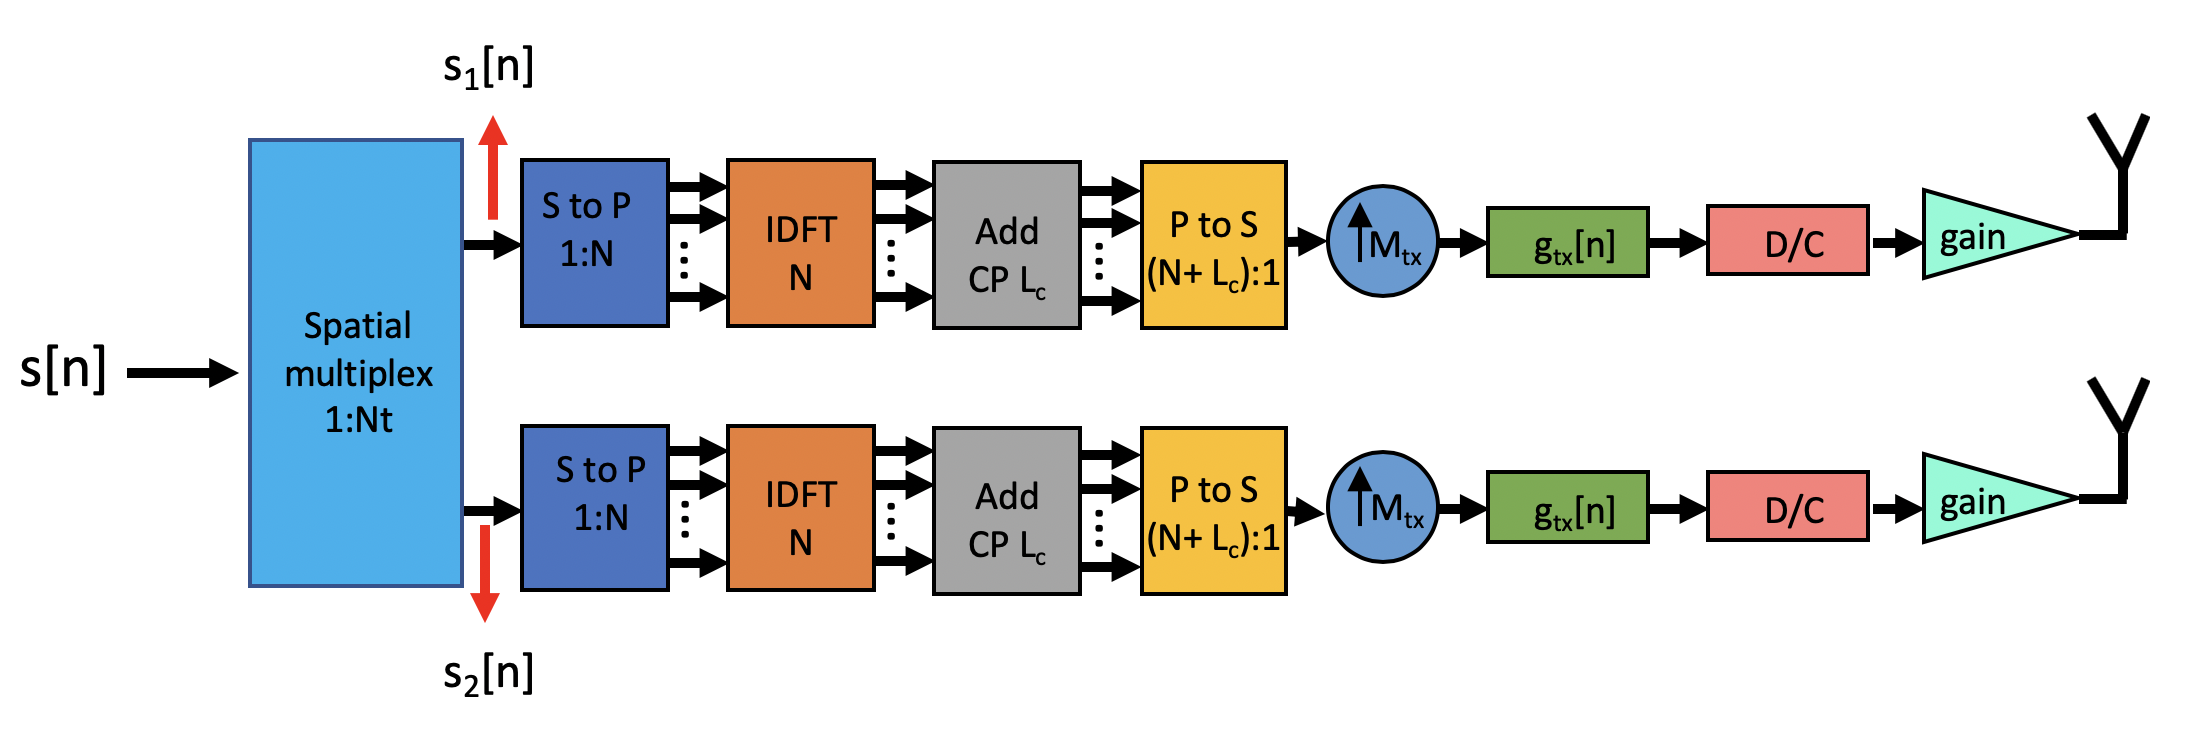
\includegraphics[width=\columnwidth]{lab11/figure2.png}
\caption{Transmitter for a 2x2 MIMO-OFDM system with spatial multiplexing.} \label{transmit}
\end{center} 
\end{figure}

\begin{figure}
\begin{center}
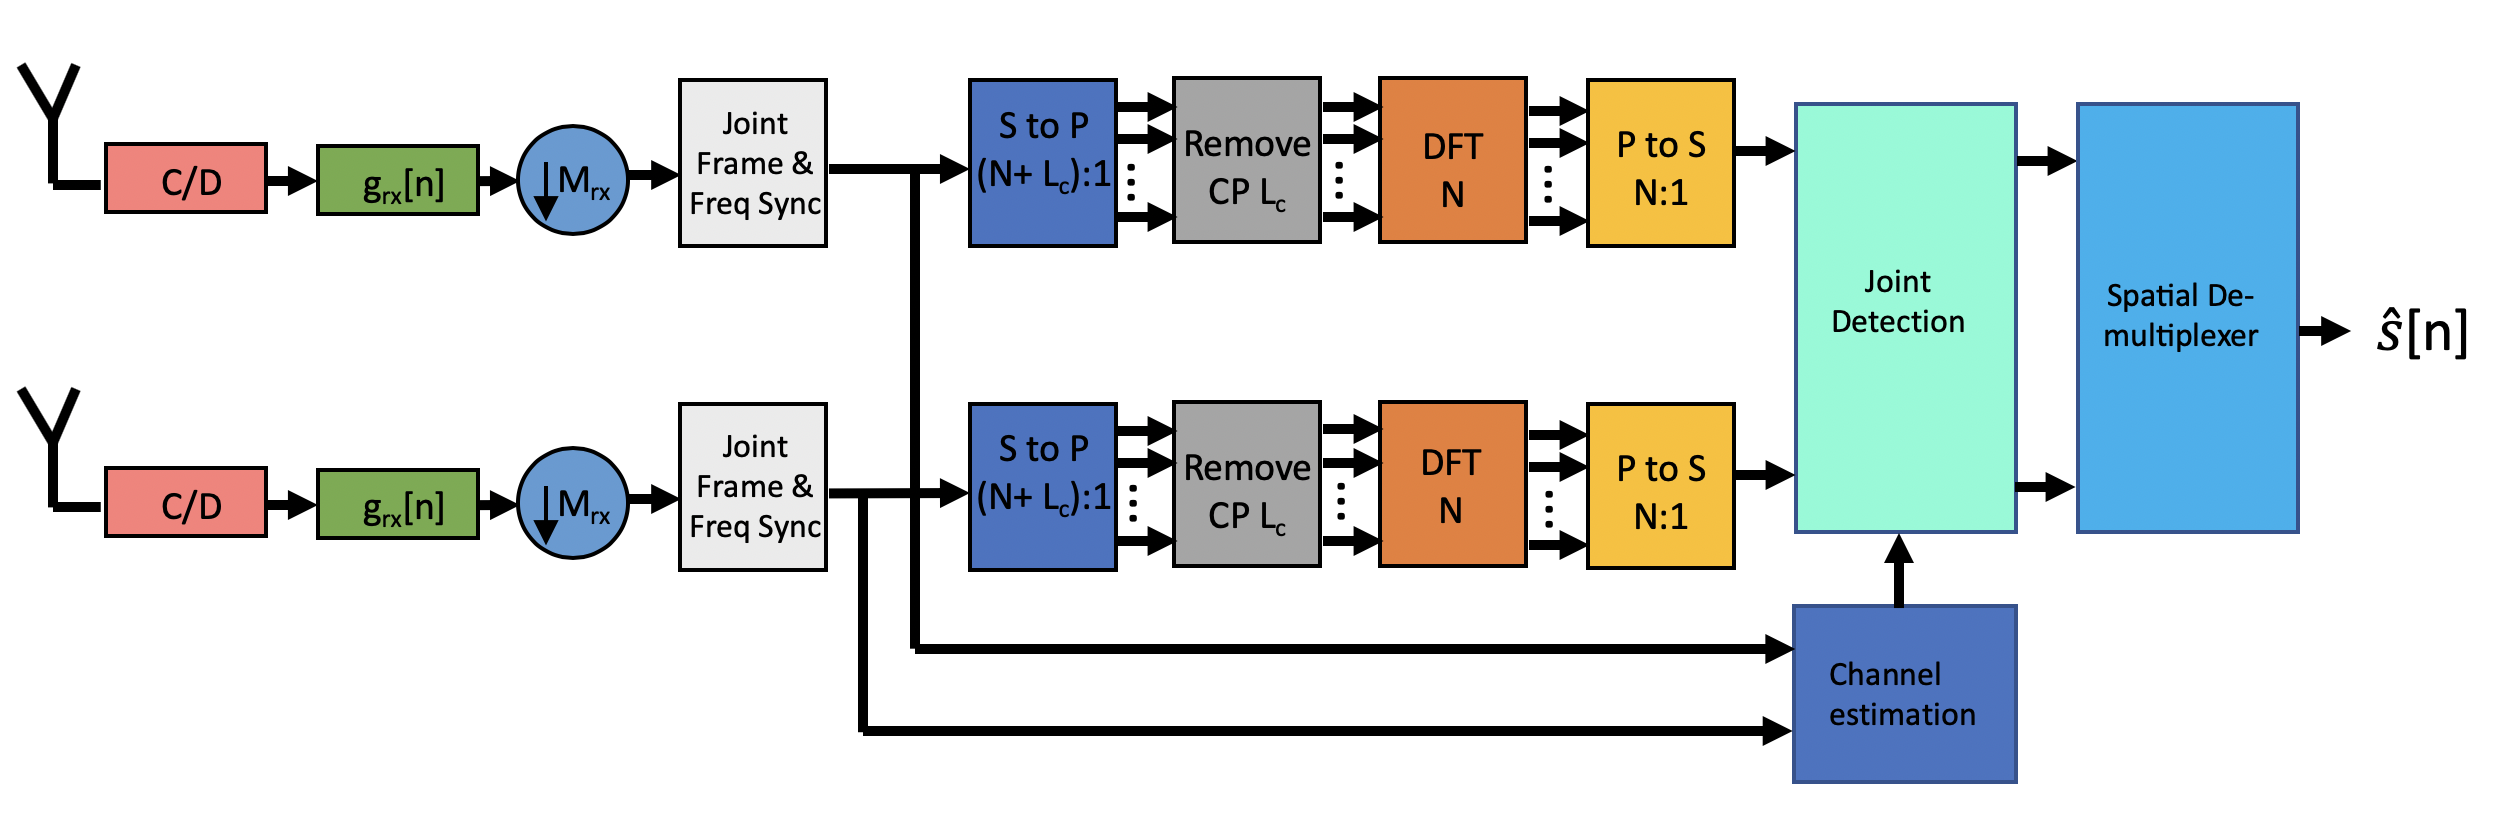
\includegraphics[width=\columnwidth]{lab11/figure3.png}
\caption{Receiver for a 2x2 MIMO-OFDM system with spatial multiplexing. The key blocks that will be implemented in this lab is channel estimation and joint detection.} \label{receive}
\end{center} 
\end{figure}

Let $\sfs[n]$ represent a single symbol stream. For the model, $\sfs[n]$ is split in to $N_t$ different sets of subsymbols after going through the spatial multiplexer where $N_t$ is the number of transmit antennas. Let $\sfs_j[n]$ represent the set of subsymbols for transmit antenna $j$. Each set of subsymbols then proceed through a SISO-OFDM system. Let $w_j[n]$ represent the time domain signal that will be sent over the channel that includes the cyclic prefix. The block diagram in Figure \ref{transmit} represents the MIMO-OFDM transmitter.

On the receive side, each receive antenna will see some combination of all transmit signals. The block diagram in Figure \ref{receive} represents the MIMO-OFDM receiver. In addition, for transmit antenna $j$ and receive antenna $i$, there is a unique channel $h_{i,j}[l]$. The signal from receive antenna $i$ can be written as:
\begin{equation}
    y_i[n] = \sum_{j=1}^{N_t}\sum_{l=0}^{L} h_{i,j}[l]w_j[n-l] + v_i[n]
\end{equation}
We will now rewrite the equation in the frequency domain. First we can take N-DFT of the channel.
\begin{equation}
    \sfh_{i,j}[k] = \sum_{l=0}^L h_{i,j}[l]e^{-j\frac{2\pi kl}{N}}
\end{equation}
Then, after removing the cyclic prefix from $w_j[n]$ and taking the N-DFT of it, we can rewrite the channel as follows:
\begin{equation}
    \sfy_i[k] = \sum_{j=1}^{N_t} \sfh_{i,j}[k]\sfs_j[k] + \sfv[k]
\end{equation}
Now, we can write this in full matrix form by stacking the receive signals $\sfy_i[k]$, the transmitted symbols $\sfs_j[k]$, and defining the full channel matrix response as $|\bsfH[k]|_{i,j} =\sfh_{i,j}[k]$.
\begin{equation}
    \bsfy[k] = \bsfH[k]\bsfs[k] + \bsfv[k]
\end{equation}
Note that $\bsfy[k]$ is size ($N_r$ by 1); $\bsfs[k]$ is size ($N_t$ by 1); $\bsfH[k]$ is size ($N_r$ by $N_t$); and $\bsfv[k]$ is size ($N_r$ by 1)

%%%%%%%%%%%%%%%%%%%%%%%%%%%%%%%%%
\subsection{OFDM Preamble}
In this section, we will discuss how we design our channel estimation field in the preamble. For the channel estimation field, we are using unique Zadoff-Chu sequences for each antenna. The Zadoff-Chu sequence is defined as follows:
\[
p[n] = 
        \begin{array}{cc}
 \Bigg\{ & 
        \begin{array}{cc}
          e^{j\frac{M\pi n^2}{N_p}} & N_p \textrm{ is even}\\ [0.5em]
          e^{j\frac{M\pi n(n+1)}{N_p}} & N_p \textrm{ is odd}
        \end{array}
    \end{array}
\]
where $N_p$ is the length of the sequence and $M$ is coprime with $N_p$. So essentially for each antenna, pick a unique number $M$ that is coprime with $N_p$. 

%%%%%%%%%%%%%%%%%%%%%%%%%%%%%%%%%
\subsection{Channel estimation}
    Once frame synchronization and the carrier frequency offset correction is complete, we can move on to channel estimation. A key component to this is that each transmit antenna needs to send unique training sequences with good correlation properties. This approach sends training over only one OFDM symbol so it is better to estimate the channels in time domain. The following derivation references \cite[Chapter 6, Section 5.4]{Hea:Introduction-to-Wireless-Digital:17}.
    
    In the frequency domain, let $\{\bsft[k]\}_{k=0}^{N-1}$ be the known training sequence and the received signal is
    \begin{equation}\label{eq1}
        \bsfy[k] = \bsfH[k]\bsft[k] + \bsfv[k], k\in [0,N-1]
    \end{equation}
    Now, we rewrite the $\bsfH[k]$ in the time domain and expand it out. 
    \begin{align}
        \bsfH[k] &= \sum_l^L \bsfH[l]e^{-j\frac{2\pi kl}{N}} \\ 
                 &= 
                 \begin{bmatrix}
                    \bH[0] & \bH[1] &  \hdots & \bH[L]
                 \end{bmatrix}
                 \begin{bmatrix}
                    \bI_{N_t} \\ 
                    e^{-j\frac{2\pi k}{N}}\bI_{N_t} \\ 
                    \vdots \\ 
                    e^{-j\frac{2\pi kL}{N}}\bI_{N_t}
                 \end{bmatrix} \\
                 &= \begin{bmatrix}
                    \bH[0] & \bH[1] &  \hdots & \bH[L]
                 \end{bmatrix}
                 (\bee[k] \otimes \bI_{N_t}) \\
   \vecc(\bsfH[k]) &= ((\bee[k]^T \otimes \bI_{N_t}) \otimes \bI_{N_r}) 
                    \begin{bmatrix}
                        \vecc(\bH[0]) \\
                        \vecc(\bH[1]) \\
                        \vdots \\ 
                        \vecc(\bH[L])
                    \end{bmatrix} \\
                &= ((\bee[k]^T \otimes \bI_{N_t}) \otimes \bI_{N_r}) \bh \label{eq2}
    \end{align}
    where 
    \begin{align}
        \bee[k] = \begin{bmatrix}
            1 & e^{-j\frac{2\pi k}{N}} & \hdots & e^{-j\frac{2\pi kL}{N}} 
        \end{bmatrix} \\ 
        \bh = \begin{bmatrix}
                        \vecc(\bH[0]) \\
                        \vecc(\bH[1]) \\
                        \vdots \\ 
                        \vecc(\bH[L])
             \end{bmatrix}
    \end{align}
    We can now plug in \ref{eq2} into \ref{eq1}:
    \begin{align}
        \bsfy[k] &= \vecc(\bsfH[k]\bsft[k]) + \bsfv[k] \\
        &= (\bsft[k]^T \otimes \bI_{N_r})\vecc(\bsfH[k]) + \bsfv[k] \\
        &=(\bee[k]^T \otimes \bsft[k]^T \otimes \bI_{N_r})\bh + + \bsfv[k] \label{eq3}
    \end{align}
    Now, by stacking all subcarriers $\cK = {k_1, k_2, ..., k_t}$,
    \begin{align}
        \bsfT &= \begin{bmatrix}
                        \bee[k_1]^T \otimes \bsft[k_1]^T \otimes \bI_{N_r} \\
                        \bee[k_2]^T \otimes \bsft[k_2]^T \otimes \bI_{N_r} \\
                        \vdots \\ 
                        \bee[k_t]^T \otimes \bsft[k_t]^T \otimes \bI_{N_r}
                    \end{bmatrix} \\ 
        \vec{\bsfy} &= \begin{bmatrix}
                \bsfy[k_1] \\ \bsfy[k_2] \\ \vdots \\ \bsfy[k_t]
        \end{bmatrix}
    \end{align}
    Now we can rewrite \ref{eq3}:
    \begin{equation}
        \vec{\bsfy} = \bsfT \bh + \bsfv
    \end{equation}
    We need enough subcarriers to make sure that $\bsfT$ is square or tall and that the training sequences are designed such that $\bsfT$ is full rank. Assuming it fits this criteria, we can compute the least squares estimate:
    \begin{equation}\label{eq4}
        \hat{\bh} = (\bsfT^*\bsfT)^{-1}\bsfT^*\vec{\bsfy}
    \end{equation}
    Lastly, to get the channel estimate in the frequency domain $\bsfH[k]$, we can plug \ref{eq4} into \ref{eq2} and reshape it so that it is not vectorized.
%%%%%%%%%%%%%%%%%%%%%%%%%%%%%%%%%
\subsection{Detection}
For this lab, we will be using a zero-forcing detector. The following derivation references \cite[Chapter 6, Section 5.2]{Hea:Introduction-to-Wireless-Digital:17}. Once the frequency domain channel estimate $\bsfH$ is computed, we define $\bsfG$ as the pseudo-inverse of $\bsfH$. Then we calculate a temporary vector $\bsfz$ for detection:
\begin{align}
    \bsfz[k] &= \bsfG[k]\bsfy[k] \\
    \hat{s}[k] &= \arg \min_{c \in \cC} |\bsfz[k] - c|^2
\end{align}
Note that $c$ is a vector of the same size of $\bsfy[k]$ and each element is a possible symbol from 4-QAM. For this lab, since there are two transmit antennas, there are a total of 16 vectors in $\cC$. Also note that when implementing this, each element in $\bsfy[k]$ refers to a symbol sent from an antenna. The intuition for detection for MIMO is to figure out which combination of symbols that goes through the channel looks most like our observation. By going through all subcarriers $k$, we can append our detected symbols together as such
    \begin{equation}
        \hat{\bs} = \begin{bmatrix}
            \hat{s}[k_1] & \hat{s}[k_2] & \hdots & \hat{s}[k_t]
        \end{bmatrix}
    \end{equation}
A row in $\hat{\bs}$ will refer to the estimate of the symbols sent from a single transmit antenna.
%%%%%%%%%%%%%%%%%%%%%%%%%%%%%%%%%
\section{Prelab}
%%%%%%%%%%%%%%%%%%%%%%%%%%%%%%%%%

This section describes what you should plan to accomplish prior to attending the lab. Your instructor may require you to turn in parts of your solution for each subsection. 

%%%%%%%%%%%%%%%%%%%%%%%%%%%%%%%%%
\subsection{Writing code to implement key functions in a MIMO-OFDM system}
Write code to implement the following operations for a system that transmits data in frames with a length $\Ntr$ cyclically prefixed Zadoff-Chu sequence with cyclic prefix size $\Lp$. Your data should also have a cyclic prefix of length $\Lc$.
\begin{itemize}
\item OFDM preamble generation. Generate the unique training sequences used for each transmit antenna and add the cyclic prefix. The structure of this function is given in the file \verb|ofdm_preamble_generator.m|.
\item Channel estimation. The structure of this function is given in the file \verb|channel_estimation.m|.
\item Symbol detection. The structure of this function is given in the file \verb|detect_symbol.m|. 
\end{itemize}

The template of all above functions are provided, you should fill in each of them. You cannot change the type and number of the input/output parameters.

\turnin{Your code.} 

%%%%%%%%%%%%%%%%%%%%%%%%%%%%%%%%%
\subsection{Testing your code}

In this part, you will vary your SNR and record the SER. The required parameters are listed in \ref{sc_tab_sys_par_simulation}. These should be already defined in \verb|transmitter.m| and \verb|receiver.m|.

Let $\{ \hat{h}[\ell,m] \}_{\ell=0}^L$ be the channel estimate in the $m$-th Monte Carlo simulation out of $M$ total simulations. The mean-squared error (MSE) is estimated as 
\begin{align}
\mathrm{MSE} & = \frac{1}{M} \sum_{m=0}^{M-1} \sum_{\ell=0}^L |  \hat{h}[\ell,m]  - h[\ell]|^2
\end{align}
This would apply to only on channel and is computed for you in \verb|receiver.m|. Report the average MSE of all channels. 
\begin{table}[h!]
	\caption{System parameters for frequency-selective channel evaluation (simulation)}
	\begin{center}
		\begin{tabular}{|c|c|c|} \hline
			Property & Variable name &Value  \\ \hline	
			Modulation scheme & \verb|M| & 4 \\ \hline
			Type of channel sequence & \verb|training_seq_name| & 'Zadoff-Chu' \\ \hline
			Repetition of training sequence & \verb|training_seq_repetition| & 1 \\ \hline
			Length of Zadoff-Chu sequence & \verb|N_ZC| & 52 \\ \hline
			Co-prime parameter with \verb|N_ZC| & \verb|M_ZC| & 3 \\ \hline
			Co-prime parameter with \verb|N_ZC| & \verb|M_ZC2| & ? \\ \hline
			Length of cyclic prefix for training $\Lp$ & \verb|L_P| & 16 \\ \hline
			Number of DFT $N$ & \verb|N_carriers| & 64 \\ \hline
			Length of cyclic prefix for data $\Lc$ & \verb|L_CP| & 16 \\ \hline			
			Channel taps & \verb|channel_taps| & $h$\\ \hline
			Carrier frequency offset & \verb|channel_cfo| & 200 \\ \hline
			Channel Delay & \verb|channel_delay| & 10$\times$2e-7 \\ \hline
			SNR & \verb|channel_snr_dB| & 1:30 dB\\ \hline
			tx rx usrp sampling rate & \verb|usrp_sample_rate| & 5 MS/s \\ \hline
			upsampling factor &  \verb|upsampling_factor| & 10   \\ \hline 
			downsamping factor &  \verb|downsampling_factor| & 10   \\ \hline 
			roll off factor $\alpha$  & \verb|roll_off| & 0.5 \\ \hline
			filter spans length & \verb|filt_spans| & 6 symbols\\ \hline
			Estimated order of channel & \verb|channel_order_estimate| & 5 \\ \hline
			total frames received & \verb|total_frames_to_receive| & 100\\ \hline
		\end{tabular}
	\end{center} \label{sc_tab_sys_par_simulation}
\end{table}

\turnin{Report your average MSE and SER for SNR ranging from 1 to 30 dB or report the plots generated after running systemcheck.m}

%%%%%%%%%%%%%%%%%%%%%%%%%%%%%%%%%
\section{Laboratory experiments}
%%%%%%%%%%%%%%%%%%%%%%%%%%%%%%%%%
%%%%%%%%%%%%%%%%%%%%%%%%%%%%%%%%%
\subsection{USRP Setup}
In this lab, we are using 4 NI-USRP 2921's, where 2 are used for transmitter and 2 are used for the receiver. Each pair of USRP's are then connected with the MIMO cable. You will need 2 instances of MATLAB to run the lab, which means you can either have one computer with 2 Ethernet cables connected to the pair of USRP's and have 2 instances of MATLAB running for the transmitter and receiver, OR have two computers running an instance of MATLAB that are connected to a specific pair of USRP's. Make sure the IP addresses for the USRP's are unique. For more information on how to test connections and set the IP address, refer to lab 2.

In addition, since there are differences between each USRP, an external clock source is necessary to sync the pair of transmitters and receivers. We are using 2 SRS Rubidium Frequency Standards (FS725) in the lab - one for each pair of USRP's. Connect the 10 MHz outputs from the FS725 to the 'ref in' of the USRP using a SMB to SMA cable which should be provided for you. Refer to Figure \ref{fs725} for an illustration of how to connect the FS725 to the USRP's.

\begin{figure}
\begin{center}
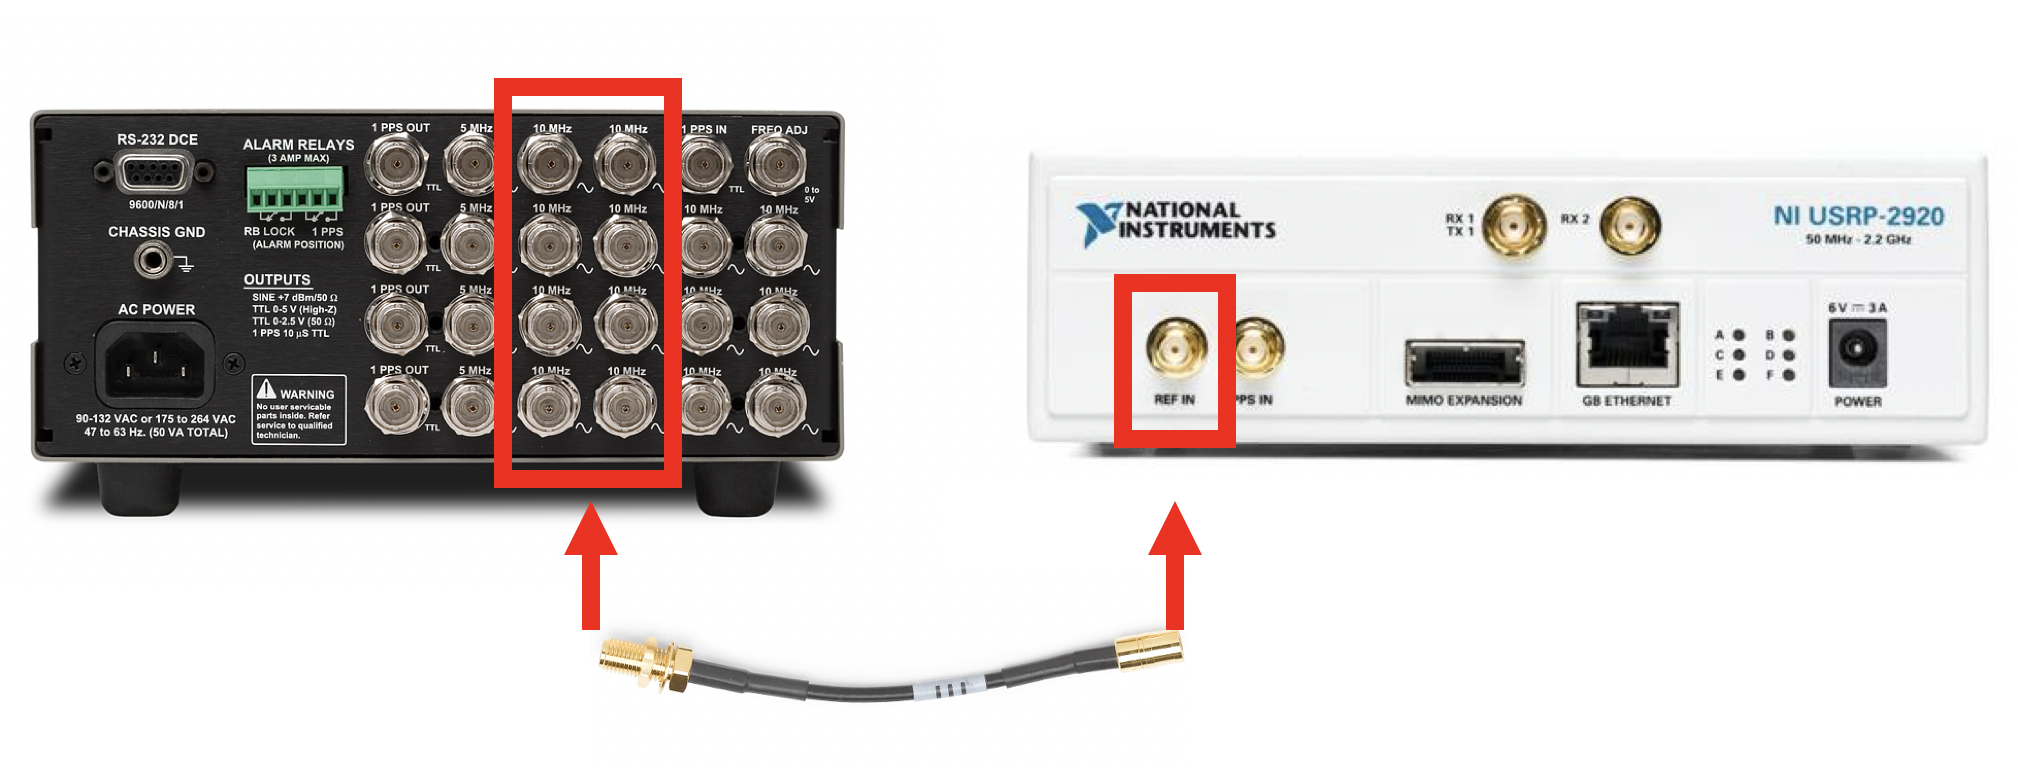
\includegraphics[width=\columnwidth]{lab11/figure1.png}
\caption{This is an illustration of how to connect the FS725 (left) and USRP 2921 (right). For the FS725, the SMB to SMA cable can be connected to any of the 8 available 10 MHz outputs. For the USRP, the SMB to SMA cable is connected to the 'ref in' plug. For the second USRP, connect it to FS725 the same way by using another SMB to SMA cable and another available 10 MHz output.} \label{fs725}
\end{center} 
\end{figure}


The system parameters used in this lab without particular declaration is given in \tabref{sc_tab_sys_par_exp}
\begin{table}[h!]
	\caption{System parameters for frequency-selective channel evaluation (simulation)}
	\begin{center}
		\begin{tabular}{|c|c|c|} \hline
			Property & Variable name &Value  \\ \hline	
			Modulation scheme & \verb|M| & 4 \\ \hline
			Type of channel sequence & \verb|training_seq_name| & 'Zadoff-Chu' \\ \hline
			Length of Zadoff-Chu sequence & \verb|N_ZC| & 52 \\ \hline
			Co-prime parameter with \verb|N_ZC| & \verb|M_ZC| & 3 \\ \hline
			Co-prime parameter with \verb|N_ZC| & \verb|M_ZC2| & ? \\ \hline
			Length of cyclic prefix for training $\Lp$ & \verb|L_P| & 16 \\ \hline
			Number of DFT $N$ & \verb|N_carriers| & 64 \\ \hline
			Length of cyclic prefix for data $\Lc$ & \verb|L_CP| & 16 \\ \hline			
			Channel Delay & \verb|channel_delay| & 10$\times$2e-7 \\ \hline
			tx rx usrp sampling rate & \verb|usrp_sample_rate| & 5 MS/s \\ \hline
			upsampling factor &  \verb|upsampling_factor| & 10   \\ \hline 
			downsamping factor &  \verb|downsampling_factor| & 10   \\ \hline 
			roll off factor $\alpha$  & \verb|roll_off| & 0.5 \\ \hline
			filter spans length & \verb|filt_spans| & 6 symbols\\ \hline
			Estimated order of channel & \verb|channel_order_estimate| & 3 \\ \hline
			total frames received & \verb|total_frames_to_receive| & 100\\ \hline
		\end{tabular}
	\end{center} \label{sc_tab_sys_par_exp}
\end{table}

%%%%%%%%%%%%%%%%%%%%%%%%%%%%%%%%%
\subsection{Experiment 1: Estimate SER Performance of your system}
%%%%%%%%%%%%%%%%%%%%%%%%%%%%%%%%%
Run your code and compute the SER for 5 iterations of 5 different SNR levels. 
\turnin{The measured SER for 5 different SNR levels}

%%%%%%%%%%%%%
\subsection{Experiment 2: Performance Comparison}
%%%%%%%%%%%%%%%%%%%%%%%%%%%%%%%%%
Compare your data to the performance of SISO-OFDM from Lab 9 or 10. Plot the average SER over SNR and compare the SISO and MIMO systems. Explain your observations.
\turnin{Overlay plot of SISO and MIMO SER over SNR and your explanation.}

%%%%%%%%%%%%%%%%%%%%%%%%%%%%%%%%%
\subsection{Experiment 3: Unplugging an Antenna}
%%%%%%%%%%%%%%%%%%%%%%%%%%%%%%%%%
Completely unscrew one transmit antenna and run your code. At high SNR, on average over 5 iterations, what is the SER? Theoretically what should the SER be and why?

\turnin{Report your expected SER, experimental SER, and explanation. }

\section{Solutions}
\subsection{Prelab}
Refer to figures \ref{prelab1} and \ref{prelab2}
\begin{figure}
\begin{center}
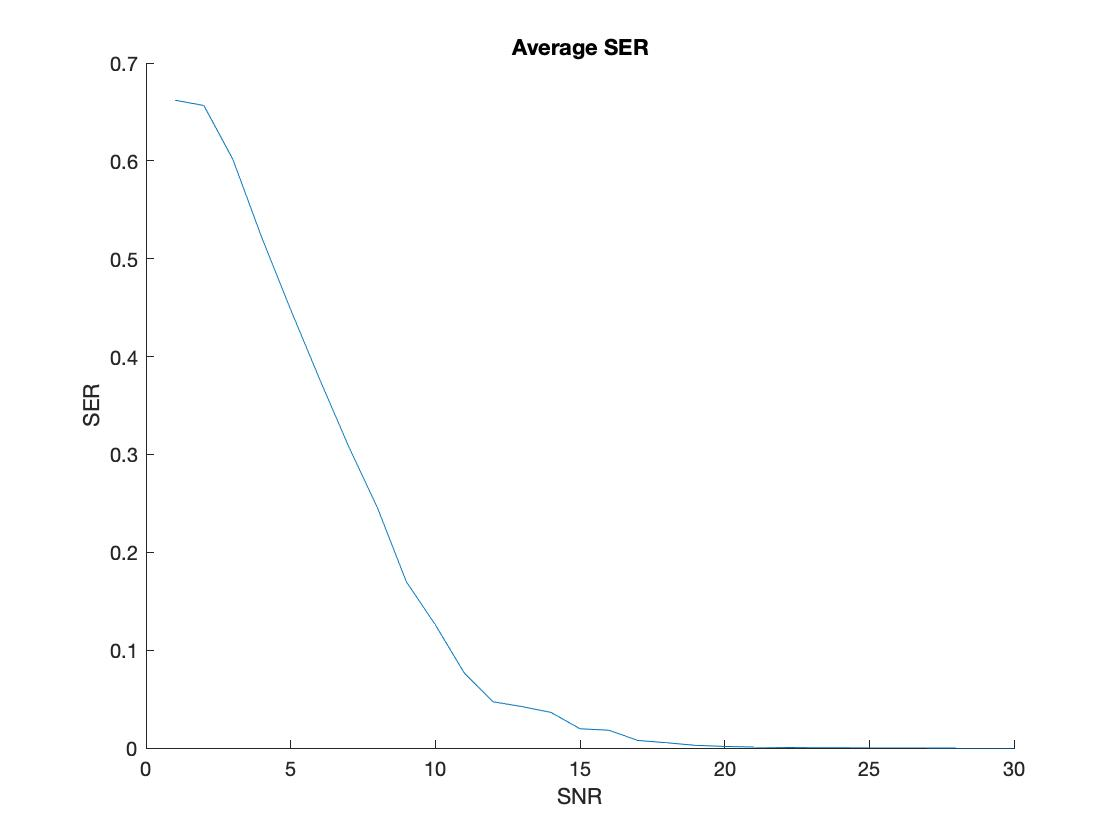
\includegraphics[width=\columnwidth]{lab11/prelab1.jpg}
\caption{Plotting the average SER over SNR for MIMO-OFDM simulation.} \label{prelab1}
\end{center} 
\end{figure}
\begin{figure}
\begin{center}
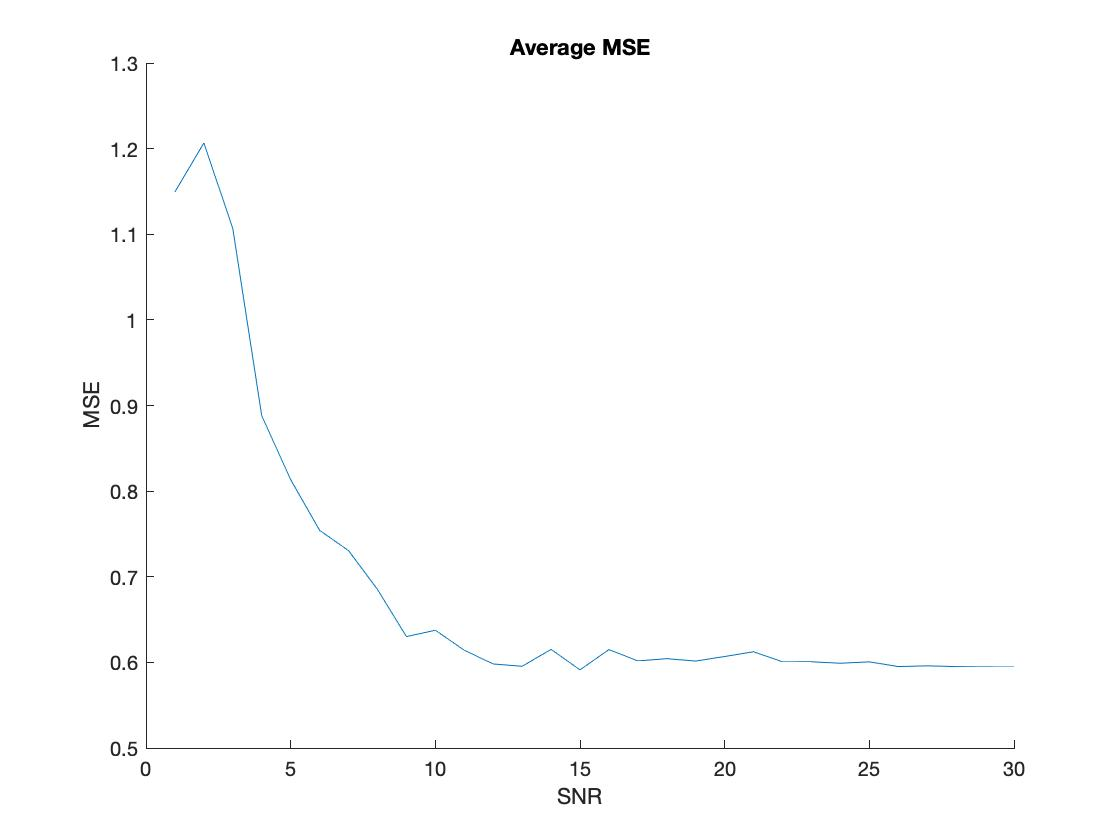
\includegraphics[width=\columnwidth]{lab11/prelab2.jpg}
\caption{Plotting the average MSE over SNR for MIMO-OFDM simulation.} \label{prelab2}
\end{center} 
\end{figure}
\subsection{Experiment 1}
    Refer to table \ref{exp1}
    \begin{table}[h!] \caption{The average SER over SNR}
        \begin{center} 
            \begin{tabular}{c|c}
                SNR & SER  \\ \hline
              0.5862   & 0.5751 \\    
              9.5031   & 0.3007   \\ 
              16.4995  & 0.1146    \\
              23.9156  & 0.0134    \\
              31.6561  & 0.0005    \\
              38.8820  & 0.0016
            \end{tabular}
        \end{center}
    \end{table} \label{exp1}
\subsection{Experiment 2}
MIMO-OFDM tends to do better at lower SNR's because of an increase in diversity gain. Refer to Figure \ref{exp2}.
\begin{figure}
\begin{center}
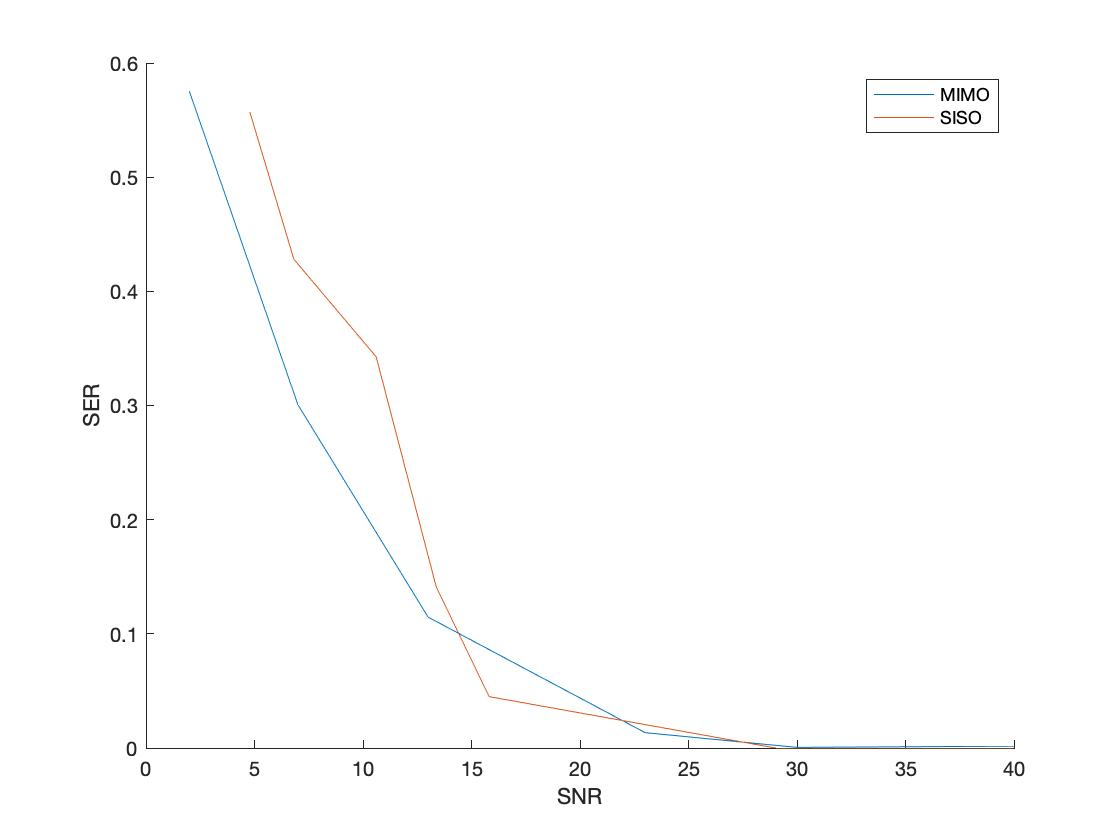
\includegraphics[width=\columnwidth]{lab11/exp2.jpg}
\caption{Plotting the average SER over SNR for MIMO-OFDM and SISO-OFDM.} \label{exp2}
\end{center} 
\end{figure}
\subsection{Experiment 3}
    The SER should average out to be 0.375 or $\frac{3}{8}$. Based on our model, one set of subsymbols should be perfectly sent. During detection, we are trying to see the best combination of two symbols that are sent through the channel. We can always detect the first symbol but the second symbol of the combination could anything. If antenna 2 is disconnected, then we can fully detect $\sfs_1[n]$ and randomly detect $sfs_2[n]$ at rate of 0.25. So in total should be 0.375.
%%%%%%%%%%%%%%%%%%%%
% Below will be deleted when we compile the whole book
% Make sure this is in the correct directory
\setlength{\baselineskip}{1pt}
\bibliographystyle{IEEEtran}
\bibliography{IEEEabrv,new_lab_refs_rwh,new_refs}
\end{document},